% !TeX root = ./main.tex
\section{Additionnal Cryptanalysis}
\label{sec:appendix-cryptanalysis}



\subsection{Algebraic Analysis}
\label{sec:cryptanalysis-algebraic}
Algebraic cryptanalysis consists of formulating nonlinear equations that an attacker can derive from the information observed in terms of the secret key material. Several techniques, such as Gröbner basis methods or linearization, exist for solving such systems of equations, and we discuss them in this section. Based on this analysis, we claim that \coolName{} is resistant to algebraic attacks and their improvements.

%A first generic approach can be to rely on a Gröbner basis. A second generic approach can be to use linearization technique, that is considering any multivariate monomial involved in the system as new and independent variable also be to and a second approach to attacks based on deriving low-degree equations in the internal state from the observation of the keystream. We also discuss linearization techniques further below.


\paragraph{Gröbner Basis.} Such an attack consists of four main steps: formulating the equations that model the intended cryptanalysis, computing their Gröbner basis, applying a ``change of monomial ordering'' to transform the Gröbner basis into a more useful form, and finally solving the result using univariate techniques. The complexity of the first and last steps is usually negligible, meaning that we should evaluate the time complexity of at least one of the other two steps.

However, as recently shown in~\cite{C:BBLAOP24}, it is possible to write the equations in such a way as to entirely bypass the computation of the Gröbner basis. This is achieved by choosing a custom \emph{monomial ordering} that ensures the equations, as formulated, immediately form a Gröbner basis. This approach can be applied here by assigning increasing weights to the successive outputs of the key schedule, so that the leading monomials in each equation involve only a single key variable. This method is effective for at least the first four clock cycles, as the clock outputs are independent.

At this stage, we have 16 independent equations of degree 15 (the degree of $\thesbox$). Adding the equations corresponding to the next $20$ clocks, we get as many equations as unknowns, which, in particular, should lead to a 0-dimensional ideal. As conjectured in~\cite{EPRINT:Perrin24}, the ideal degree of this system can be lower-bounded by $15^{16} \approx 2^{62.5}$. This bound would be exact if the 80 remaining equations somehow failed to contribute to an increase in this quantity, or if the ideal degree was in some way decreased by one of these equations (despite the 0-dimension). Given that change of order algorithms are at least quadratic in the ideal degree, we can safely claim security against Gröbner-basis-based algebraic attacks.

%\paragraph{Classical Algebraic Attack.} \lp{todo. On dit qu'on s'en fout parce que faire 0 dans $\mainField$ ça dit pas grand chose?}\yr{Oui, on s'en fout}


\paragraph{Linearization.}Such attacks may, a priori, pose a threat, as they have led to the downfall of two \gls{FHE}-friendly stream ciphers, namely {\tt FLIP}~\cite{EC:MJSC16} and {\tt Elisabeth}~\cite{AC:CHMS22}, which were broken in~\cite{C:DuvLalRot16} and~\cite{AC:GBJR23}, respectively. The structure of these ciphers made such attacks an inherent risk: in both cases, a low-degree function is applied to a constant key register to generate keystream words.  As a result, in these ciphers, the nonlinear equations derived from the keystream sequence have a constant degree. Considering all monomials (or linear combinations of monomials) as new independent variables in this representation enables powerful attacks~\cite{C:DuvLalRot16,AC:GBJR23}. These attacks are the result of  two fundamental weaknesses: the constant degree of the system and low diffusion, as the registers are never updated, only a bit-permutation is applied at each clock cycle.

These issues are directly addressed in the design of \coolName{}. First, the round function of the FSM applies the \gls{S-box} \( \thesbox \) to every digit. This \gls{S-box} has a univariate representation in \( \mainField \) that is both dense and of degree 15. Furthermore, the content of the FSM accumulates high-degree equations within the key-LFSR. As a result, the multivariate polynomial representation of the keystream digits will not have a constant degree; instead, it will be very dense and of high degree.


\paragraph{Using Annihilators.} Another powerful technique is to directly use an annihilator of the filtering function, where this annihilator has a lower degree than the original function~\cite{EC:CouMei03,C:Courtois03}. This allows the attacker to collect and solve a system of equations with a smaller degree than the original one. That is, similar to Gröbner basis-like attacks, this approach operates on the ideal generated by the polynomials. In the case of \coolName{}, we can argue and defend the role of the whitening LFSR \( \whitening \). Indeed, this LFSR has a length of 32 digits, meaning that an annihilator at the output must consider the sum of 8 outputs by \( \phi \) and cancel them with a polynomial. Therefore, without additional information, such an annihilator would need to multiply approximately 32 digits, leading to an increase in the degree. This strategy must also account for the degree increase in successive outputs of \( \phi \), as discussed above.

\paragraph{Other Techniques.}
Last but not least, algebraic attacks can be improved in several ways using the Guess-and-Determine strategy or the so-called Hybrid approach in Gröbner basis computations. In our case, one could guess key-register cells, whitening-key cells, or cells in the FSM. Although this is a valid approach, the remaining equations (depending on the guessing strategy) would either have an increased degree or require guessing too many cells, making the attack impractical.



\subsection{Comparison With {\tt LEX}}
\label{sec:security-lex}

{\tt LEX}~\cite{SAC:Biryukov06} is a stream cipher designed by Biryukov in 2006 and selected to the third phase of the eSTREAM competition. {\tt LEX} employed a rather unusual design for a stream cipher, based on the {\tt \gls{AES}} block cipher and a technique called \emph{leak extraction}. The idea of the leak extraction is to produce the key stream by extracting parts of the underlying block cipher state.

The description of {\tt LEX} is very simple and elegant. It is based on a slightly tweaked version of the {\tt \gls{AES}} where the {\sf AddRoundKey} operation before the first round is omitted and where the {\tt MixColumns} of the last round is not. For simplicity, we will still refer to this tweaked version as {\tt \gls{AES}}. First, the publicly known $IV$ is encrypted by the {\tt \gls{AES}} under the secret key $K$ to produce an initial state  $S = {\tt \gls{AES}}_K(IV)$. Then, the state $S$ is repeatedly encrypted using the OFB mode and the same secret key $K$. At each round of encryption, four words of the internal state are extracted to compose the key stream produced by {\tt LEX}. The positions of the extracted words depend on the round number and are depicted in Figure~\ref{fig:lex}.

\begin{figure}
  \centering
  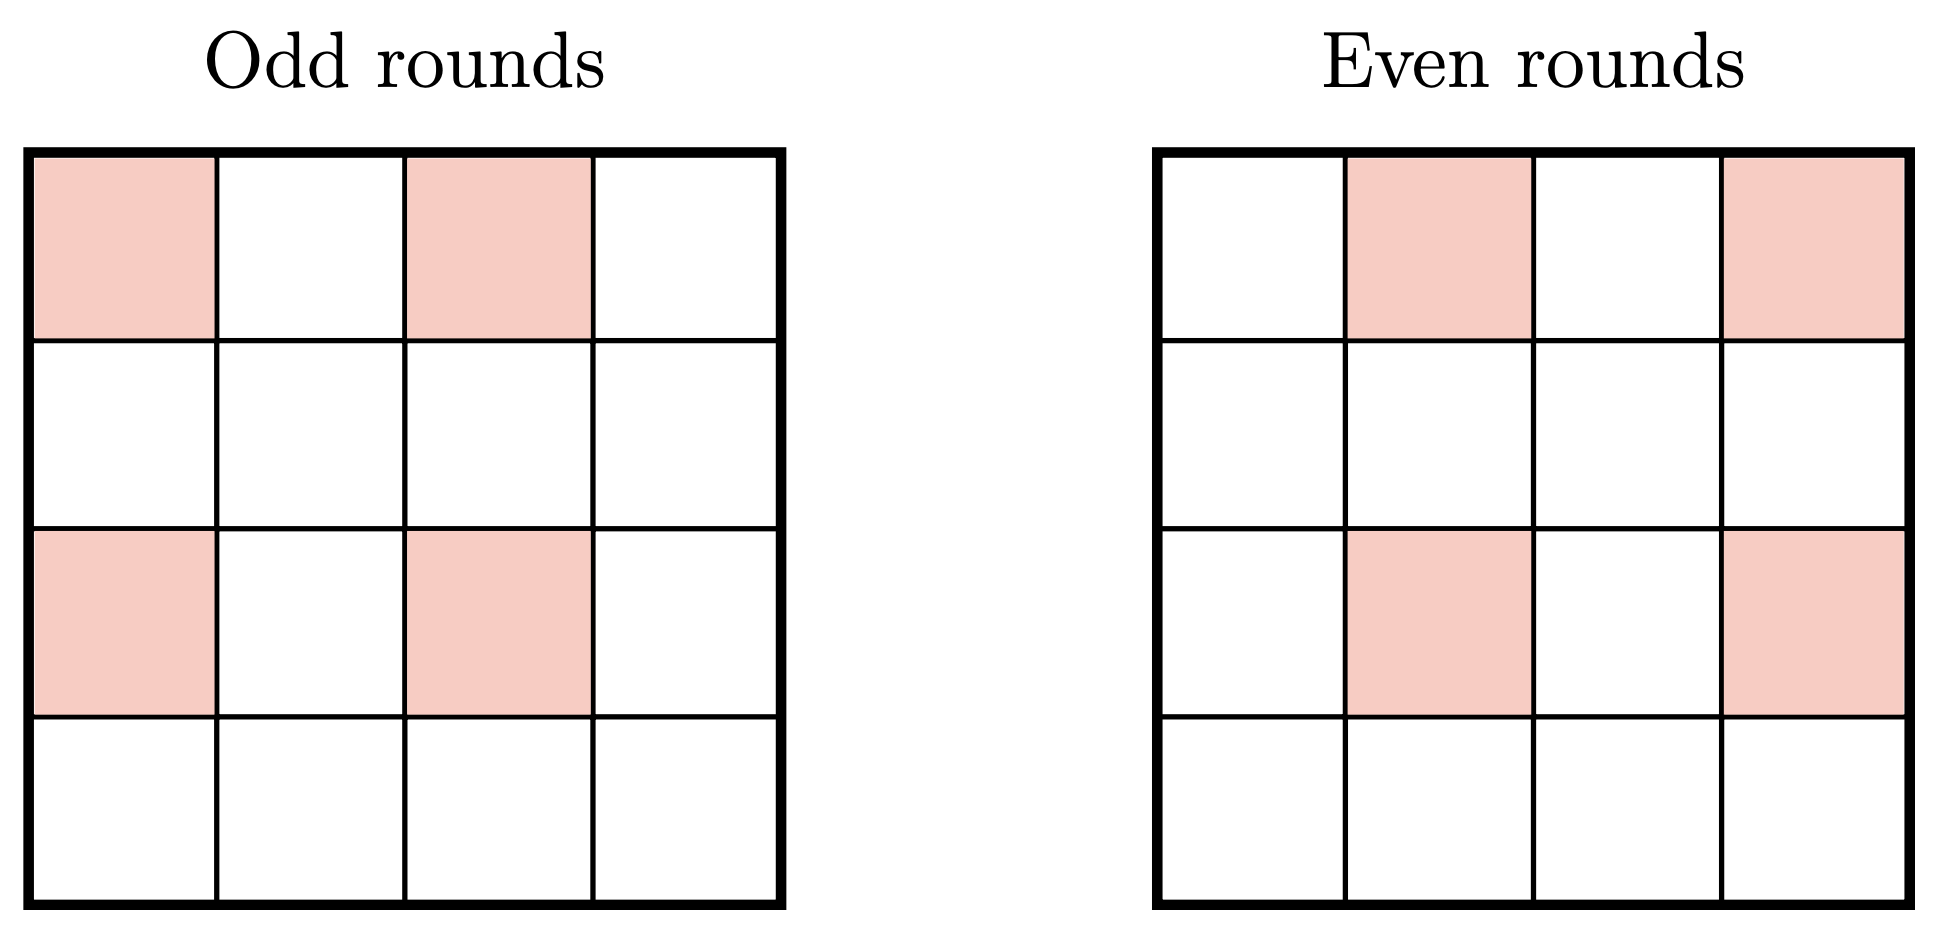
\includegraphics[width=7cm]{figures/lex.png}
  \caption{Extraction of internal state words for odd and even rounds of {\tt LEX}\label{fig:lex}. The extracted words are the ones being colored.}
\end{figure}

In 2008, Dunkelman and Keller presented an attack against LEX~\cite{AC:DunKel08b} able to recover the 128-bit secret key with $2^{36.3}$ bytes of key-stream produced by the same key and a time complexity of $2^{112}$ simple operations. This attack worked by exploiting a particular difference pattern of probability $2^{-64}$ in the {\tt \gls{AES}} internal state that could be detected by observing a $32$-bit condition in the output key stream.  The attack can be decomposed  in the three following steps:
\begin{enumerate}
\item  The attacker observes the output stream for a specific 32-bit pattern to occur (the four output words at a certain round should all be zero). This potentially indicates a special difference pattern (8 particular words with zero-difference) in the internal state of {\tt \gls{AES}}. 
\item Once this difference pattern is detected, the attacker recovers the values of 16 bytes of the internal state in both {\tt \gls{AES}} encryptions. This is achieved by guessing the difference in eight additional state words and by exploiting simple properties of the  {\sf MixColumns} and the  \gls{S-box}. 
\item Finally, using the recovered 16 bytes, the attacker proceeds with a guess-and-determine approach to retrieve the secret key. The key step here is exploiting relations derived from the {\tt \gls{AES}-128} key schedule that link bytes from three consecutive subkeys, reducing the number of required guesses to just two subkey bytes. This limits the guessing process to only 10 bytes (80 bits) in total.
\end{enumerate}

\coolName{}'s structure ressembles {\tt LEX} in several aspects, the most notable being the extraction of four words at each iteration. Additionally, \coolName{}'s round function is inspired by the {\tt \gls{AES}} round function. For these reasons, it is natural to question whether the attack described in~\cite{AC:DunKel08b} could be adapted to \coolName{}. However, as we will argue next,  \coolName{} differs from {\tt LEX} in some crucial design choices, making the Dunkelman and Keller attack very difficult to apply:

\begin{itemize}
\item The output of the FSM at every round is masked by the whitening LFSR $\mathcal{W}$ making it hard to directly recover the values of the internal state as done in the attack of {\tt LEX}.
\item The LFSR $\mathcal{K}$ playing the role of the key schedule, produces uncorrelated outputs, making it hard to find simple relations between key values in consecutive rounds. A crucial element in the success of the attack against {\tt LEX} was exactly the fact that by guessing only two key bytes, the attacker was able to recover many more key values by exploiting such relations holding over several rounds. As we showed in the previous sections, it is not possible for an attacker to extract any information on the secret key by observing the output of the FSM over 3 or 4 consecutive rounds. 
\end{itemize}


\subsection{Truncated Linear Trails from MILP}
\label{sec:milp}


In order to find a lower bound for the number of \gls{S-box}es active in a linear trail over 4 rounds of \coolName, we apply the approach introduced by Mouha \emph{et al.\@}~\cite{add:MWGP11} in the most direct way. As we are interested in the (in)activity of the Sboxes throughout the rounds, we only need to assign binary variables to output digits, but also to internal digits of the state before the \gls{S-box} layer, and before the MixColumn operation. For each round, we then have $4 + 16 + 16 = 36$ binary variables that are related one to others by the following constraints.
\begin{description}
\item[3-fork constraint.] Any output digit corresponds to a digit of the internal state after the \gls{S-box} layer, so it is naturally related to the activity of a digit before MixColumn, by taking care of the reorganization of the digits through ShiftRows. But because the activity pattern is unchanged through the \gls{S-box} layer, it is also related to a digit before the \gls{S-box} layer. The constraint between three such variables is that if one is active, then at least two of them are. This corresponds to a 3-fork constraint that can be modeled as in \cite[Sec~ 2.2]{add:MWGP11}.
\item[MDS constraint.] A given column before and after MixColumns are related by the following MDS constraint: if a digit is active, then at least 5 of them are. This can be modeled in a manner similar to the 3-fork. In our case, the binary variables associated to the state after MixColumns at round $r$ are the one corresponding to the state before the \gls{S-box} layer at round $r+1$.
\item[Border constraints.] We also add some border constraints to ensure that the initial inner state is fully inactive, and that the same holds for the final inner state. This way, we make sure that the considered linear equations do not depend on the unknown FSM state, but only on the key and output digits. We also impose that at least a digit among the ones output at the first round, and at least one among the ones of the last round must be active.
\end{description}
Finally, with the described constraints, the objective is to minimize the number of active Sboxes, that is, the number of active digits before the \gls{S-box} layer. Note that any solution to this problem is actually a worst-case scenario in our case: a returned activation pattern is not guaranteed to be actually instantiable. We solved this simple MILP model using the SageMath interface for Mixed Integer Linear Programing solving within seconds on a standard laptop. Our code is 
\ifeprint
  available online.\footnote{\url{https://github.com/CryptoExperts/Transistor/}}
\else
  provided as supplementary material.
\fi

Most notably, we have found that
\[w_4 \geq 13,\  w_5 \geq 20 \mbox{ and } w_6 \geq 25\]
with the potential trail examples depicted on Fig.~\ref{fig:trails}.
We also verified that \(w_n \geq 26\) for $n \in \{7, 8, \ldots 26\}$.
For larger values of $n$, either a trail has at least one active \gls{S-box} per
round, or it splits into two smaller trails with at least 13 active
Sboxes.  Therefore, we deduce that \(w_n \ge 26\) for all $n \ge 7$.

\begin{figure}[h]
  \centering
  \begin{subfigure}[t]{0.22\textwidth}
    \centering
    \includegraphics[scale=.55]{figures/solution_0.pdf}
    \caption{4-round trail.}
  \end{subfigure}
  \hfill
  \begin{subfigure}[t]{0.22\textwidth}
    \centering
    \includegraphics[scale=.55]{figures/solution_1.pdf}
    \caption{4-round trail.}
  \end{subfigure}
  \hfill
  \begin{subfigure}[t]{0.22\textwidth}
    \centering
    \includegraphics[scale=.55]{figures/solution_2.pdf}
    \caption{4-round trail.}
  \end{subfigure}
  \hfill
  \begin{subfigure}[t]{0.22\textwidth}
    \centering
    \includegraphics[scale=.55]{figures/solution_3.pdf}
    \caption{4-round trail.}
  \end{subfigure}
  
  \begin{subfigure}[t]{0.45\textwidth}
    \centering
    \includegraphics[scale=.6]{figures/milp_5.pdf}
    \caption{5-round trail.}
  \end{subfigure}
  \caption{Activity patterns for linear trails over 4 and 5 rounds.}
  \label{fig:trails}
\end{figure}

%\ac{Donner les figures des 4 trails tronques pour \(4\) tours ici.}


% Leo: ce qui suit est pour qu'emacs compile bien l'article, pas touche !
%%% Local Variables:
%%% mode: latex
%%% ispell-local-dictionary: "english"
%%% TeX-master: "main"
%%% End:
